\documentclass[uplatex,dvipdfmx,titlepage]{jsarticle}
\usepackage[dvipdfmx]{graphicx}
\usepackage{amsmath,amssymb}
\usepackage{bm}
\usepackage{enumitem} 
\usepackage{float}

%レポート作成に関する注意
%レポートには実験の目的、内容、実験方法、実験結果、結果に関する吟味・考察、予想との乖離があるならその原因の考察を自分の言葉でまとめる

\title{固体力学の実験}
\author{京都大学工学部物理工学科 1025363386 伊藤温大}
\date{\today}

\begin{document}
\maketitle

% --------------------------------------------------
% 目次
\tableofcontents
\clearpage
% --------------------------------------------------

\section{はじめに}
本レポートでは超音波計測による弾性波伝搬速度と弾性係数の評価についてその結果、実験課題について報告する。

% ==================================================
% 実験2（超音波計測）
% ==================================================
\section{超音波計測による弾性波伝搬速度と弾性係数の評価}

\subsubsection*{実験1}
金属ブロックに縦波および、横波の超音波を送信、受信することによって測定波形から伝搬速度を求めた。
この際、以下のような実験装置を使用した。
\begin{itemize}[nosep]
    \item 超音波送受信装置
    \item トランスデューサー
    \item 音響結合媒質
    \item 試験片
    \item ディジタルオシロスコープ
    \item パーソナルコンピューター
\end{itemize}
具体的に試験片として以下の材料を用いた。
\begin{itemize}[nosep]
    \item 機械構造用炭素鋼鋼材 S25C
    \item 機械構造用炭素鋼鋼材 S45C
    \item アルミニウム合金 A5052
    \item アルミニウム合金 A2024(超ジュラルミン)
\end{itemize}

\subsection{実験方法}
1. 試験片の寸法を測定し、記録した。この時同様の材質について4回測定し、平均をとった。記録した試験片の寸法は以下の表のようになった。

\begin{table}[H]
    \centering
    \begin{tabular}{lccc}
    \hline
    S25C & S45C & A5052 & A2025 \\ \hline
    9.882 & 9.873 & 9.98 & 10.061 \\ \hline
    \end{tabular}
\end{table}

2. 試験片を厚さ方向に複数回伝搬した波形について、それぞれの反射波の到着時刻を求めた。この時S25Cの縦波について初めの波は超音波送受信装置から出た波を観測してしまっていると考えられる。

縦波について、受信したデータはS25Cから順に以下図のようになった。

\begin{figure}[H]
    \centering
    \begin{minipage}[b]{0.48\textwidth}
        \centering
        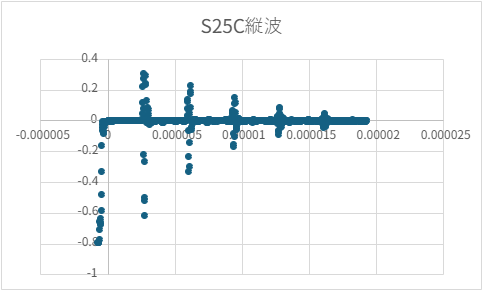
\includegraphics[width=\textwidth]{S25C縦波.png}
        \caption{S25C 縦波}
    \end{minipage}
    \hfill
    \begin{minipage}[b]{0.48\textwidth}
        \centering
        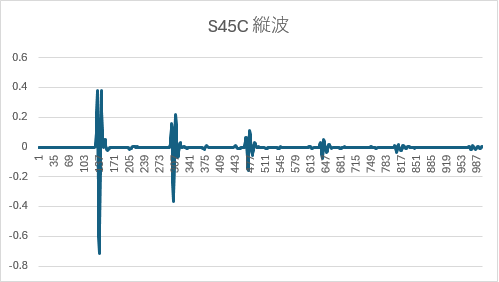
\includegraphics[width=\textwidth]{S45C縦波.png}
        \caption{S45C 縦波}
    \end{minipage}
    \\ \vspace{5mm}
    \begin{minipage}[b]{0.48\textwidth}
        \centering
        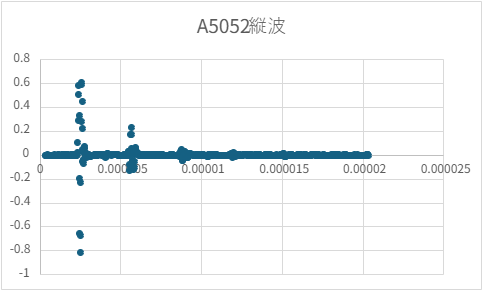
\includegraphics[width=\textwidth]{A5052縦波.png}
        \caption{A5052 縦波}
    \end{minipage}
    \hfill
    \begin{minipage}[b]{0.48\textwidth}
        \centering
        \includegraphics[width=\textwidth]{A2024.png}
        \caption{A2024 縦波}
    \end{minipage}
\end{figure}

この反射波の到着時刻を求める際には波の下限のピークの値を到着時刻として統一した。この時縦波における到着時刻はS25Cから順に以下の表のようになった。

\begin{table}[H]
    \centering
    \caption{S25C 縦波の到着時刻}
    \begin{tabular}{lcc}
    \hline
    個数 & 到着時刻 & 総距離 \\ \hline
    1つ目 & 0.00000274 & 0.019764 \\
    2つ目 & 0.00000606 & 0.039528 \\
    3つ目 & 0.0000094  & 0.059292 \\
    4つ目 & 0.00001272 & 0.079056 \\
    5つ目 & 0.00001606 & 0.09882  \\ \hline
    \end{tabular}
\end{table}

\begin{table}[H]
    \centering
    \caption{S45C 縦波の到着時刻}
    \begin{tabular}{lcc}
    \hline
    個数 & 到着時刻 & 総距離 \\ \hline
    1つ目 & 0.00000274 & 0.019746 \\
    2つ目 & 0.00000608 & 0.039492 \\
    3つ目 & 0.00000944 & 0.059238 \\
    4つ目 & 0.00001278 & 0.078984 \\ \hline
    \end{tabular}
\end{table}

\begin{table}[H]
    \centering
    \caption{A5052 縦波の到着時刻}
    \begin{tabular}{lcc}
    \hline
    個数 & 到着時刻 & 総距離 \\ \hline
    1つ目 & 0.0000025  & 0.01996 \\
    2つ目 & 0.00000558 & 0.03992 \\
    3つ目 & 0.00000884 & 0.05988 \\ \hline
    \end{tabular}
\end{table}

\begin{table}[H]
    \centering
    \caption{A2024 縦波の到着時刻}
    \begin{tabular}{lcc}
    \hline
    個数 & 到着時刻 & 総距離 \\ \hline
    1つ目 & 0.00000264 & 0.020122 \\
    2つ目 & 0.00000578 & 0.040244 \\
    3つ目 & 0.00000892 & 0.060366 \\
    4つ目 & 0.00001206 & 0.080488 \\
    6つ目 & 0.0000152  & 0.10061  \\
    7つ目 & 0.0000185  & 0.120732 \\ \hline
    \end{tabular}
\end{table}

このとき伝搬速度は以下の表のようになった。(m/s)
\begin{table}[H]
    \centering
    \begin{tabular}{lccc}
    \hline
    S25C & S45C & A5052 & A2025 \\ \hline
    5935.1 & 5897.8 & 6294.8 & 6361.5 \\ \hline
    \end{tabular}
\end{table}

横波について、観測したオシロスコープの値は以下の図のようになった。

\begin{figure}[H]
    \centering
    \begin{minipage}[b]{0.48\textwidth}
        \centering
        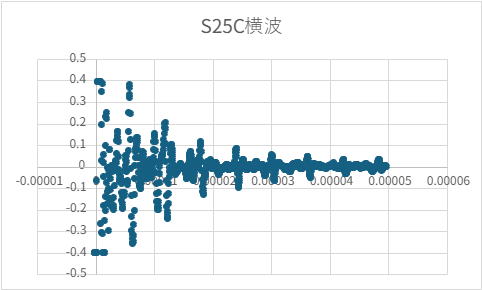
\includegraphics[width=\textwidth]{S25C 横波.png}
        \caption{S25C 横波}
    \end{minipage}
    \hfill
    \begin{minipage}[b]{0.48\textwidth}
        \centering
        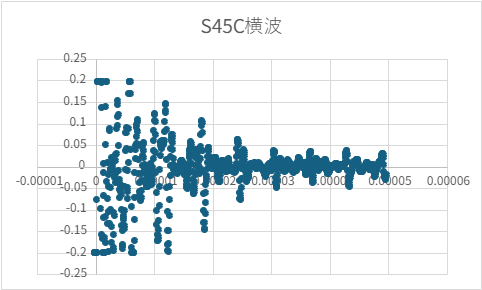
\includegraphics[width=\textwidth]{S45C横波.png}
        \caption{S45C 横波}
    \end{minipage}
    \\ \vspace{5mm}
    \begin{minipage}[b]{0.48\textwidth}
        \centering
        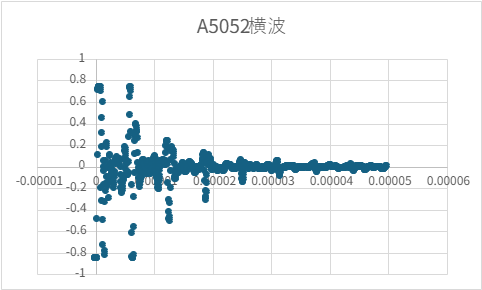
\includegraphics[width=\textwidth]{A5052横波.png}
        \caption{A5052 横波}
    \end{minipage}
    \hfill
    \begin{minipage}[b]{0.48\textwidth}
        \centering
        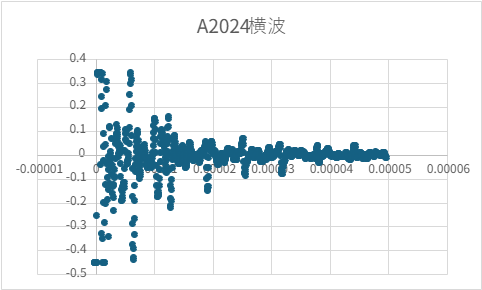
\includegraphics[width=\textwidth]{A2024横波.png}
        \caption{A2024 横波}
    \end{minipage}
\end{figure}

到着時刻はS25Cから順に以下の表のようになった。この際、1, 2回目などの波が不安定になっている点については考慮せず、安定に観測できている波について観測した。この時横波における到着時刻は波の下限のピークの値を到着時刻として統一した。

\begin{table}[H]
    \centering
    \caption{S25C 横波の到着時刻}
    \begin{tabular}{lcc}
    \hline
    個数 & 到着時刻 & 総距離 \\ \hline
    4つ目 & 2.45E-05 & 0.079056 \\
    5つ目 & 3.05E-05 & 0.09882  \\
    6つ目 & 3.67E-05 & 0.118584 \\
    7つ目 & 4.27E-05 & 0.138348 \\ \hline
    \end{tabular}
\end{table}

\begin{table}[H]
    \centering
    \caption{S45C 横波の到着時刻}
    \begin{tabular}{lcc}
    \hline
    個数 & 到着時刻 & 総距離 \\ \hline
    3つ目 & 1.86E-05 & 0.059238 \\
    4つ目 & 2.47E-05 & 0.078984 \\
    5つ目 & 3.1E-05  & 0.09873  \\
    6つ目 & 3.72E-05 & 0.118476 \\ \hline
    \end{tabular}
\end{table}

\begin{table}[H]
    \centering
    \caption{A5052 横波の到着時刻}
    \begin{tabular}{lcc}
    \hline
    個数 & 到着時刻 & 総距離 \\ \hline
    2つ目 & 6.25E-06 & 0.03992 \\
    3つ目 & 1.26E-05 & 0.05988 \\
    4つ目 & 1.88E-05 & 0.07984 \\ \hline
    \end{tabular}
\end{table}

\begin{table}[H]
    \centering
    \caption{A2024 横波の到着時刻}
    \begin{tabular}{lcc}
    \hline
    個数 & 到着時刻 & 総距離 \\ \hline
    2つ目 & 6.4E-06  & 0.040244 \\
    4つ目 & 1.91E-05 & 0.080488 \\
    5つ目 & 2.56E-05 & 0.10061  \\ \hline
    \end{tabular}
\end{table}

これによって伝搬速度は以下のようになった。
\begin{table}[H]
    \centering
    \begin{tabular}{lccc}
    \hline
    S25C & S45C & A5052 & A2024 \\ \hline
    3245.3 & 3189.9 & 3180.9 & 3154.6 \\ \hline
    \end{tabular}
\end{table}

3. 実験1によって導かれる各材料のヤング率とポアソン比を求めると以下の表のようになった。
\begin{table}[H]
    \centering
    \begin{tabular}{lcc}
    \hline
    材料 & $E$ & $\nu$ \\ \hline
    S25C  & 211.4107036 & 0.286745546 \\
    S45C  & 205.2874965 & 0.293253799 \\
    A5052 & 75.27726346 & 0.328543453 \\
    A2024 & 74.50623148 & 0.336952484 \\ \hline
    \end{tabular}
\end{table}

4. 受信した反射波形に含まれる周波数成分を、高速フーリエ変換により確認した。

\subsubsection*{実験2}
1. 送信トランスデューサと受信トランスデューサの間隔を変化させながら、波の到達時刻を調べた。この時送信トランスデューサと受信トランスデューサの間隔は2, 4, 6, 8 cmについてそれぞれ波の到達時刻を調べた。
この時観測した波は以下のようになった。

この時、それぞれの材料におけるそれぞれの間隔の到達時刻は以下のようになった。

2. トランスデューサ間の間隔と到達時刻との関係から伝搬速度を求めると以下のようになった。

実験2において測定されたRayleigh波と実験1における横波速度とPoisson比によるReyleigh波の速度との関係は以下のようになった。
\begin{table}[H]
    \centering
    \resizebox{\textwidth}{!}{
    \begin{tabular}{lccccc}
    \hline
          & Poisson比 & 横波速度   & Rayleigh波(実験1) & Rayleigh波(実測値) & 誤差(\%)   \\ \hline
    S25C  & 0.2868   & 3245.3 & 3004.238       & 2959.8         & 1.479173 \\
    S45C  & 0.2933   & 3189.9 & 2956.068       & 2953.9         & 0.073331 \\
    A5052 & 0.3285   & 3180.9 & 2964.019       & 2951           & 0.439247 \\
    A2024 & 0.337    & 3154.6 & 2943.287       & 2869.8         & 2.496754 \\ \hline
    \end{tabular}
    }
\end{table}


\subsubsection*{考察課題}
1. 超音波測定に用いた4種類の材料に対して、ヤング率/密度として定義されている比剛性を求めると、、、
、、、、、、

2. 超音波測定に用いた炭素鋼S25CとS45Cの違い、およびアルミニウム合金A5052とA2024の違いを図書で調べると、、、、、、、

\subsection{結果}

\subsection{考察}

% ==================================================
% まとめと参考文献
% ==================================================
\section{総括}
本実験を通して、光弾性法および超音波計測を用いた固体力学の評価手法について...

\section*{参考文献}
\begin{enumerate}[label={[\arabic*]}]
    \item 著者名, 『書籍名』, 出版社, 発行年.
    \item 物理工学科 実験指導書, 2026.
\end{enumerate}

\end{document}